\section{Aufbau und Durchf"uhrung}
	\label{sec:durchfuehrung}

\subsection{Kennlinienschar einer Hochvakuumdiode} % (fold)
\label{sub:subsection_name}

F"ur Aufgabenteil a wird die Versuchsapparatur nach Abb. \ref{aufgabe_a} aufgebaut.
Die Heizspannung $V_\mathrm{f}$ und der Heizstrom $I_\mathrm{f}$ wird konstant gehalten.
Die Anodenspannung wird nun variiert und der Anodenstrom abgelesen.
Aus diesen ergiebt sich die Diodenkennlinie.

Dies wird f"ur f"unf insgesamt verschiedene Heizstr"ome und -spannungen wiederholt.

In Aufgabenteil b wird die h"ochste Heizspannung genutzt.


\begin{figure}[!h]
	\centering
	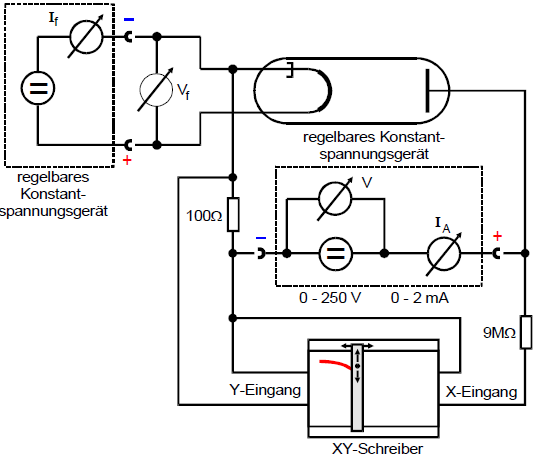
\includegraphics[width = 10cm]{img/aufgabea.PNG}
	\caption{Schaltung zum Aufnehmen von Diodenkennlinien}
	\label{aufgabe_a}
\end{figure}

\subsection{Anlaufstrom} % (fold)
\label{sub:anlaufstrom}

In Aufgabenteil c wird das Anlaufstromgebiet der Diode untersucht.
Daf"ur wird eine Schaltung nach Abb. \ref{aufgabe_c} aufgebaut, wobei auf ein paar Dinge zu achten ist.
Da die Str"ome sehr gering sind muss zwischen Anode und Eingangsbuchse ein m"oglichst kurzes Kabel benutzt werden.
Zudem ist der "Ubergangswiderstand durch mehrmaliges Drehen des Bananensteckers in seiner Buchse zu minimieren.

\begin{figure}[!h]
	\centering
	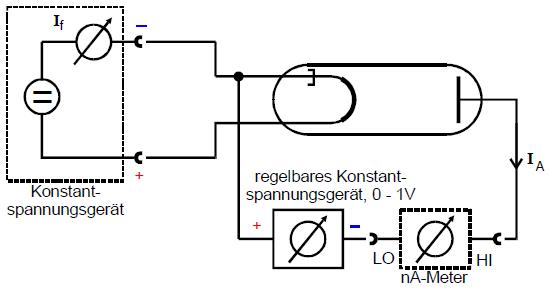
\includegraphics[width = 10cm]{img/aufgabec.PNG}
	\caption{Schaltung zur Aufnahme einer Anlaufstromkurve}
	\label{aufgabe_c}
\end{figure}